\subsection{Effizienz}
\label{bpr:effizienz}

Im Bezug auf die Effizienz des hier beschriebenen Algorithmus muss zwischen der asymptotischen Worst-Case Analyse und der Effizienz in realen Anwendungsszenarien unterschieden werden. Es existieren bereits andere Verfahren mit sehr guten theoretischen Laufzeitschranken von \(\Theta(n)\) \cite{saca:9} (DC3, \cref{algorithm:dc3}) sowie praxisnähere Algorithmen mit einer Laufzeitkomplexität von \(\O(n \log n)\) \cite{saca:5} (DivSufSort, \cref{algorithm:divsufsort}), wobei \(n\) die Länge des Eingabestrings ist. Da es aber in der Praxis durchaus vorstellbar ist, dass Algorithmen mit schlechterer asymptotischer Laufzeit für reale Anwendungszwecke schneller sind, werden wir uns in \cref{ergebnisse} mit praktischen Laufzeitmessungen im Vergleich zu anderen Algorithmen auseinandersetzen.\par
Gerade in der Praxis ist allerdins nicht nur die Laufzeitkomplexität, sondern auch die Speicherkomplexität von hoher Bedeutung. Die nachfolgende Analyse beschäftigt sich daher insbesondere auch mit dem Speicherbedarf des \bpr-Algorithmus.

\subsubsection{Worst-Case Analyse}
\label{bpr:effizienz:theorie}

Die Worst-Case Analyse des Algorithmus kann für beide Phasen separat erfolgen, da die asymptotische Schranke nur durch die schlechtere Schranke der beiden Phasen festgelegt wird. Wir betrachten daher zunächst die Speicher- und Laufzeitkomplexität der ersten Phase, bevor wir die zweite Phase auf ähnliche Art und Weise untersuchen. Für die angegebenen Laufzeitschranken gibt die Größe \(n\) dabei immer die Länge des Eingabestrings an.
\paragraph*{Phase 1}
In der ersten Phase des Algorithmus wird die initiale Einteilung der Suffixe in Level-\(d\)-Buckets bestimmt. Gemäß der Beschreibung von Schürmann und Stoye wird dazu eine Tabelle \bkt (s.~Abbildung \ref{fig:bkt}) angelegt. Bedingt durch die Größe des Alphabets und die Länge \(d\) der Präfixe fällt auf, dass die Tabelle Speicher in der Größe von \(\O(|\Sigma|^d)\) benötigt. Unter der Annahme, dass die Allokation von Speicher der Größe \(n\) einen Laufzeitaufwand von \(\Theta(n)\) verursacht, bildet die Speicherkomplexität zugleich eine untere Schranke für die Laufzeitkomplexität. Dennoch geben Schürmann und Stoye in ihrer Analyse eine Worst-Case Laufzeit von \(\O(n)\) für die erste Phase an \cite[Kapitel 3.2]{schuermann2005}. Um zumindest in der Theorie eine lineare Laufzeit in Abhängigkeit von \(n\) zu garantieren, kann angenommen werden, dass \(|\Sigma|\) und \(d\) konstant oder zumindest unabhängig von \(n\) sind. Falls \(d\) allerdings von \(n\) abhängig gewählt wird, so sind einige andere Faktoren entscheidend, auf welche im Folgenden eingegangen wird.\par
Zunächst ist zu beachten, dass nicht der gesamte allokierte Speicher auch verwendet werden muss: Die Verarbeitung der Eingabe erfolgt laut Dokumentation des Algorithmus in dieser Phase in einer konstanten Anzahl von Iterationen über den Eingabestring\footnote{Laut Schürmann und Stoye \cite[Kapitel~3.3]{schuermann2005} besteht die erste Phase von \bpr lediglich aus drei Iterationen über den Eingabestring, was eine lineare Laufzeitschranke zur Folge hat. Bei genauerer Betrachtung der im Rahmen der Publikation veröffentlichten Implementierung (abrufbar unter \url{http://bibiserv.techfak.uni-bielefeld.de/bpr/}) fällt allerdings auf, dass tatsächlich auch eine vollständige Iteration über das Array \bkt stattfindet, welche die Laufzeitschranke auf \(\O(|\Sigma|^d)\) anhebt. Diese Iteration wird jedoch weder in der Beschreibung des Algorithmus erwähnt, noch in der zugehörigen Analyse berücksichtigt.} \inputtext bzw. \inputtextplus. Obwohl das Array \bkt Platz für alle möglichen Präfixe der Länge \(d\) bietet, müssen nur die Einträge verwendet werden, zu denen tatsächlich entsprechende Teilstrings in \inputtextplus existieren. Die Anzahl solcher Präfixe ist allerdings durch \(\O(n\)) beschränkt, woraus eine lineare Laufzeit resultiert, sofern es die Implementierung erlaubt, Speicher beliebiger Größe in konstanter Zeit zu allokieren.\par
Alternativ ist auch die Verwendung einer geeigneten Hashtabelle denkbar, um den exponentiellen Speicherbedarf zu vermeiden. Ein solcher Ansatz bietet -- wenn auch im ursprünglichen Algorithmus nicht vorgesehen -- für große Alphabete schon bei kleiner Konstante \(d\) die einzige Möglichkeit, den Algorithmus auf gängiger Hardware angemessen speicherschonend betreiben zu können.
\paragraph*{Phase 2}
Für die asymptotische Laufzeit der zweiten Phase wurde von Schürmann und Stoye nur eine auf groben Abschätzungen basierende Schranke von \(\O(n^2)\) angegeben \cite[Kapitel~3.2]{schuermann2005}. Die entsprechende Analyse beruht auf der Annahme, dass in jeder Ebene der Rekursion insgesamt höchstens \(n\) Suffixe sortiert werden müssen, was eine Laufzeit von \(\O(n \log n)\) zur Folge habe. Da die Anzahl der Rekursionsebenen offensichtlich durch \(\frac n d\) beschränkt ist (bedingt durch die Erhöhung von \offset um \(d\) pro Ebene), sei die Laufzeit der gesamgen Phase durch \(\O(\frac n d \cdot n \log n)\) beschränkt. Es wird außerdem angegeben, dass eine Schranke von \(\O(n^2)\) erreicht werden kann, wenn \(d = \log n\) gesetzt wird.\par\smallskip
Wir wollen uns diese Laufzeitschranke genauer ansehen. Zunächst fällt auf, dass für den Sortiervorgang in Phase 2 die Algorithmen \emph{Insertionsort} und \emph{Quicksort} verwendet werden. \emph{Insertionsort} hat bekanntermaßen sowohl im besten Fall, als auch im durchschnittlichen Fall eine Laufzeit von \(\O(n^2)\). Da dieser Algorithmus allerdings nur für Buckets der Größe 15 oder kleiner verwendet wird, ist in diesem Fall \(n\) durch 15 nach oben beschränkt, woraus sogar eine konstante Laufzeit resultiert. Interessanter ist die Analyse bei \emph{Quicksort}: Zwar beträgt die Laufzeit dieses Verfahrens im durchschnittlichen Fall \(\O(n \log n)\), im schlechtesten Fall kann die Laufzeit allerdings auch bis auf \(\O(n^2)\) ansteigen. In einer Worst-Case Analyse muss also streng genommen eine quadratische Laufzeitschranke für den Sortiervorgang angenommen werden. Die von Schürmann und Stoye angenommene asymptotische Schranke von \(\O(n \log n)\) kann tatsächlich erreicht werden, wenn für den Sortiervorgang \emph{Mergesort} oder \emph{Heapsort} verwendet wird. Da es in der Praxis dennoch vorteilhaft sein kann, \emph{Quicksort} zu verwenden \cite[Tabelle~1]{quicksort}, ist es hier vertretbar, die Sortiervorgänge mit diesem Algorithmus durchzuführen und anzumerken, dass eine asymptotische Laufzeitschranke von \(\O(n \log n)\) zumindest mit alternativen Sortieralgorithmen \emph{möglich} ist. Wir gehen daher auch in der weiteren Analyse davon aus, dass Sortieren in \(\O(n \log n)\) möglich ist.\par
Hervorzuheben ist auch die Wahl von \(d = \log n\), um insgesamt eine Laufzeit von \(\O(n^2)\) zu erhalten. Den Parameter \(d\) in Abhängigkeit von \(n\) zu wählen, ist zwar grundsätzlich möglich, steht aber im Gegensatz zur in Phase 1 aufgestellten Annahme, \(d\) sei konstant. Betrachten wir nur konstante Werte für \(d\), so fällt der Faktor \(\frac 1 d\) in \(\O(\frac n d \cdot n \log n)\) weg und wir erhalten eine Worst-Case Laufzeit von \(\O(n^2\log n)\).\par\smallskip
Obwohl es mit der oben angewandten Methode zur Abschätzung der Laufzeit, welche sich auf die Tiefe der Rekursion und den maximalen Aufwand pro Ebene bezieht, scheinbar nicht möglich ist, kleinere obere Schranken als \(\O(n^2 \log n)\) zu finden, konnte noch keine einfache Beispieleingabe gefunden werden, die tatsächlich eine derart hohe Laufzeit verursacht. Die größte Schwierigkeit dabei ist, dass der Algorithmus vergleichsweise undurchsichtig die Abhängigkeiten zwischen den Suffixen verwendet.
\paragraph*{Gesamter Algorithmus}
In den beiden vorangegangenen Abschnitten wurde die Laufzeit der beiden Phasen einzeln analysiert. Eine Laufzeitschranke für den Gesamten Algorithmus ergibt sich durch das Maximum beider Komponenten. Da es aber für eine präzise Angabe notwendig ist, die Wahl des Parameters \(d\) festzulegen, betrachten wir zuerst einige Optionen. Im Vorfeld wurde bereits diskutiert, welche Auswirkungen auf die Laufzeit die Wahl von \(d = \log n\) im Gegensatz zu einem konstanten Wert für \(d\) hat. Diese Unterschiede zeigt Tabelle~\ref{table:time_bounds}.
\begin{table}[h]
	\centering
    \resizebox{\textwidth}{!}{
        \begin{tabular}{|l|l|l|l|}
            \hline
                Phase & \(d\) konstant & \(d = \log n\) & \(d = \log_{|\Sigma|}n\) \\
                \hline
                \hline
                Phase 1 & \(\O(|\Sigma|^d)\) & \(\O(|\Sigma|^{\log n}) = \O(n^{\log |\Sigma|})\) & \(\O(|\Sigma|^{\log_{|\Sigma|} n}) = \O(n^{\log_{|\Sigma|} |\Sigma|}) = \O(n)\) \\
                Phase 2 & \(\O(n^2 \log n)\) & \(\O(n^2)\) & \(\O\left(\frac{n^2 \log n}{\log_{|\Sigma|}n}\right) = \O(n^2 \log |\Sigma|)\) \\
                \hline
                Gesamt & \(\O(|\Sigma|^d + n^2 \log n)\) & \(\O(n^{\max\{2, \log |\Sigma|\}})\) & \(\O(n^2 \log |\Sigma|)\)\\
                \hline
        \end{tabular}
    }
    \vspace{1ex}
    \caption{Laufzeitschranken für \bpr in Abhängigkeit von \(d\)}
    \label{table:time_bounds}
\end{table}
Für einen konstanten Wert \(d\) haben wir bereits in den beiden teilweisen Analysen gesehen, dass die Laufzeit polynomiell in \(|\Sigma|\) und \(n\) ist. Allerdings ist festzustellen, dass sich bereits für kleine \(d\) eine sehr hohe reale Laufzeit ergeben kann. Für den Fall \(d = \log n\), welcher von Schürmann und Stoye gewählt wurde, ist die Laufzeit zwar für feste Alphabetgrößen \(|\Sigma|\) polynomiell in \(n\). Für allgemeine Alphabete jedoch ist die Laufzeit nicht polynomiell.\par
Ein möglicher Ansatz um eine in \(n\) und \(|\Sigma|\) polynomielle Laufzeitschranke zu erreichen kann gefunden werden, wenn \(d\) in Abhängigkeit der Alphabetgröße \(|\Sigma|\) und der Eingabelänge \(n\) als \(d = \log_{|\Sigma|} n\) gewählt wird. Da auf diese Option bisher noch nicht eingegangen wurde, sind in Tabelle~\ref{table:time_bounds} auch die separaten Schranken für die erste und zweite Phase angegeben. Der Parameter \(d\) ist hier so gewählt, dass das exponentielle Wachstum in Phase 1, wie es für \(d = \log n\) auftritt, vermieden werden kann, wodurch dort eine asymptotische Laufzeit von \(\O(n)\) erreicht wird. Die Laufzeit für die zweite Phase ist zwar etwas schlechter als für \(d = \log n\), da aber \(|\Sigma| \leq n\) gilt, wird hier zumindest eine bessere Laufzeit erzielt, als für ein konstantes \(d\).

%\subsubsection{Praktische Laufzeitmessungen}
\label{bpr:effizienz:praxis}

Bisher wurden mit Ausnahmen von \emph{Quicksort} nur asymptotische Laufzeitschranken thematisiert, welche in der praktischen Anwendung eine geringere Rolle spielen, als in der theoretischen Analyse.
In der Praxis kann es vorkommen, dass gerade für sehr kleine Eingaben Algorithmen mit schlechterer asymptotischer Laufzeit schnellere Ergebnisse liefern als vermeintlich effizientere Algorithmen mit besseren Laufzeitschranken.
Der wesentliche Grund dafür liegt darin, dass in der Analyse in \(\O\)-Notation konstante Faktoren in der Laufzeit nicht berücksichtigt werden. Das führt dazu, dass der gewünschte Vorteil in der tatsächlichen Laufzeit effizienter Algorithmen mitunter erst bei Eingabegrößen auftritt, wie sie in der Realität selten oder gar nicht auftreten.\par\smallskip
Im Rahmen der Projektgruppe \emph{SACABench} wollen wir uns mit realen Anwendungsszenarien auseinandersetzen. Es liegt daher nahe, ausgewählte Algorithmen nicht nur in der Theorie, sondern auch im praktischen Einsatz zu evaluieren und mit anderen Algorithmen zu vergleichen. Da die Erstellung von Suffixarrays besonders in der Bioinformatik Anwendung findet, können für praktische Laufzeitmessungen Eingaben gewählt werden, die für dieses Gebiet typisch sind und es in vergleichbarer Art und Weise repräsentierten. Für die Evaluation von \bpr (\emph{bpr}) haben Schürmann und Stoye daher einige DNA-Sequenzen gewählt, anhand derer sie den von ihnen entwickelten Algorithmus testen \cite[Kapitel~4]{saca:2}. Die Auswahl der Sequenzen ist in Tabelle \ref{table:genomes} zu sehen und umfasst verschiedene -- in diesem Anwendungsgebiet häufig sehr geringe -- Alphabetgrößen und Eingabelängen. Bei den hier aufgeführten Testdaten handelt es sich um einen Auszug der in der ursprünglichen Publikation verwendeten Daten.\par
\begin{table}[h]
	\resizebox{\textwidth}{!}{
		\begin{tabular}{|l|r|r|r|r|l|}
			\hline
			\multicolumn{1}{|c|}{\multirow{2}{*}{data set}} & \multicolumn{2}{c|}{LCP} & \multicolumn{1}{c|}{\multirow{2}{*}{\makecell{string\\length}}} & \multicolumn{1}{c|}{\multirow{2}{*}{\makecell{alphabet\\size}}} & \multicolumn{1}{c|}{\multirow{2}{*}{description}} \\
			\cline{2-3}
			& average & maximum & & & \\
			\hline
			\hline
			\emph{E. coli} genome & 17 & 2815 & 4,638,680 & 5 & \emph{Escherichia coli} genome \\
			\emph{A. thaliana} chr. 4 & 58 & 30,319 & 12,061,490 & 7 & \emph{A. thaliana} chromosome 4 \\
			\emph{Human} chr. 22 & 1,979 & 199,999 & 34,553,758 & 5 & \emph{H. sapiens} chromosome 22 \\
			\emph{C. elegans} chr. 1 & 3,181 & 110,283 & 14,188,020 & 5 & \emph{C. elegans} chromosome 1 \\
			\hline
			6 \emph{Streptococci} & 131 & 8,091 & 11,635,882 & 5 & 6 \emph{Streptococcus genomes} \\
			4 \emph{Chlamydophila} & 1,555 & 23,625 & 4,856,123 & 6 & 4 \emph{Chlamydophila} genomes \\
			3 \emph{E. coli} & 68,061 & 1,316,097 & 14,776,363 & 5 & 3 \emph{E. coli} genomes \\
			\hline
		\end{tabular}
	}
	\vspace{1ex}
	\caption[Beschreibung des Testdatensatzes]{Beschreibung des Testdatensatzes. Übernommen aus \cite[Tabelle~1]{saca:2}.}
	\label{table:genomes}
\end{table}
\noindent Die Auswertung erfolgte auf einem \emph{1.3 GHz Intel Pentium\texttrademark~M} Prozessor mit 512\,MB Arbeitsspeicher. Verglichen wurde der \bpr Algorithmus dabei mit anderen in der Praxis relevanten Verfahren (s.~Tabelle~\ref{table:construction_times}), wobei die jeweils beste im Test erreichte Laufzeit visuell hervorgehoben ist.
\begin{table}[h]
	\resizebox{\textwidth}{!}{
		\begin{tabular}{|l|r|r|r|r|r|r|r|r|}
			\hline
			\multicolumn{1}{|c|}{\multirow{2}{*}{\makecell{DNA sequences}}} & \multicolumn{8}{c|}{construction time (sec.)} \\
			\cline{2-9}
			& \multicolumn{1}{c|}{\emph{bpr}} & \makecell{\emph{deep}\\\emph{shallow}} & \multicolumn{1}{c|}{\emph{cache}} & \multicolumn{1}{c|}{\emph{copy}} & \multicolumn{1}{c|}{\emph{qsufsort}} & \makecell{\emph{difference}\\\emph{cover}} & \makecell{\emph{divide}\\\emph{conquer}} & \multicolumn{1}{c|}{\emph{skew}} \\
			\hline
			\hline
			\emph{E. coli} genome & \textbf{1.46} & 1.71 & 3.69 & 2.89 & 2.87 & 4.32 & 5.81 & 13.48 \\
			\emph{A. thaliana} chr. 4 & 5.24 & \textbf{5.01} & 12.24 & 9.94 & 8.42 & 13.29 & 16.94 & 38.30 \\
			\emph{Human} chr. 22 & \textbf{15.92} & 16.64 & 40.08 & 30.04 & 26.52 & 44.93 & 51.31 & 112.38 \\
			\emph{C. elegans} chr. 1 & \textbf{5.70} & 6.03 & 20.79 & 17.48 & 13.09 & 16.94 & 18.64 & 41.28 \\
			\hline
			6 \emph{Streptococci} & \textbf{5.27} & 5.97 & 14.43 & 10.38 & 13.16 & 14.50 & 16.40 & 36.24 \\
			4 \emph{Chlamydophila} & \textbf{2.31} & 3.43 & 17.46 & 14.45 & 7.49 & 5.59 & 6.13 & 14.13 \\
			3 \emph{E. coli} & \textbf{8.01} & 13.75 & 437.18 & 1294.30 & 32.72 & 20.57 & 21.58 & 47.32 \\
			\hline
		\end{tabular}
	}
	\vspace{1ex}
	\caption[Konstruktionszeiten für Suffixarrays diverser DNA-Sequenzen mit verschiedenen Algorithmen]{Konstruktionszeiten für Suffixarrays diverser DNA-Sequenzen mit verschiedenen Algorithmen (\bpr mit \(d = 7\)). Übernommen aus \cite[Tabelle~2]{saca:2}.}
	\label{table:construction_times}
\end{table}
Es ist gut zu erkennen, das für die hier getesteten Fälle \emph{bpr} im Vergleich zu anderen Verfahren sehr gute Ergebnisse zeigt. Selbst für den Fall von \emph{A. thaliana}, wo die schnellste Laufzeit von \emph{deep shallow} erreicht wird, ist \emph{bpr} nur geringfügig langsamer. Weitere Tests -- unter anderem mit geschriebener Sprache und künstlich generierten Strings -- zeigen außerdem, dass neben der Länge des Strings und der Alphabetgröße auch die Länge des längsten gemeinsamen Präfixes (\emph{longest common prefix, LCP}) einen entscheidenden Einfluss auf die Laufzeiten der Algorithmen hat: So ist die tatsächliche Laufzeit von \emph{bpr} für geringe LCP vergleichbar mit \emph{deep shallow}, \emph{cache} und \emph{copy}, für steigende LCP ist \emph{bpr} allerdings der schnellste getestete Algorithmus \cite[Kapitel~4]{saca:2}. Bei den hier aufgeführten Ergebnissen ist außerdem zu beachten, dass die getesteten Verfahren dem Stand des Jahres 2005 entsprechen. Neuere Algorithmen wie beispielsweise von Nong, Zhang und Chan \cite{saca:6}, die mit linearen Laufzeitschranken auch in der Praxis sehr gute Ergebnisse erzielen, wurden bisher nicht unter vergleichbaren Konditionen getestet.\par\smallskip
Ferner ist zumindest am Rande zu anzumerken, dass für die hier nicht aufgeführten Tests auf größeren Alphabeten ein geringerer Wert für den Parameter \(d\) gewählt wurde. Die Wahl geschah scheinbar ausschließlich in Abhängigkeit von der Alphabetgröße \(|\Sigma|\) und unabhängig von der Textlänge \(n\). Da auf diese Eigenschaft in den durchgeführten Tests nicht eingegangen wurde, handelt es sich dabei allerdings nur um eine augenscheinliche Vermutung.

\subsubsection{Unterschiede zur Referenzimplementierung}
\label{bpr:effizienz:modifikationen}

Die Implementierung des \bpr Algorithmus für das \sacabench Framework erfolgte in erster Linie entlang der im Paper \cite{saca:2} beschriebenen Variante des Algorithmus. Daraus ergaben sich zunächst einige strukturelle Unterschiede des Quellcodes im Vergleich zur Referenzimplementierung des Autors. Erst nach der Fertigstellung einer lauffähigen und stabilen Implementierung wurden dann die von Schürmann beschriebenen Modifikationen \cite[Kapitel 3]{saca:2} implementiert, die zur Verbesserung der praktischen Laufzeit beitragen sollen, ohne die asymptotische Laufzeit zu beeinflussen.\par
Erst im Anschluss daran fand ein direkter Vergleich der beiden Implementierungen statt, der einige algorithmische Unterschiede in der Umsetzung von Teilfunktionen offenbarte. Teilweise konnte die Laufzeit durch Anpassung derartiger Codestellen an das Original verringert werden, während sich in anderen Funktionen die neu implementierte Variante als effizienter herausstellte. In allen Fällen wurde dann jeweils die schnellere Methode beibehalten. Die wichtigsten dadurch entstandenen Unterschiede zwischen der Referenzimplementierung und derer der Projektgruppe werden in diesem Kapitel aufgeführt.

\paragraph{Seward's copy}
\label{bpr:seward}
Beide Varianten des Algorithmus verwenden die von Seward \cite{seward2000} beschriebene Copy-Technik, um aus bereits sortierten Einträgen die Reihenfolge von bis dahin unsortierten Suffixen abzuleiten. 
\begin{figure}[ht]
	\resizebox{\textwidth}{!}{
		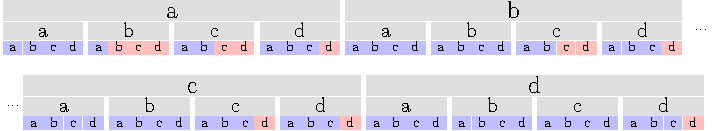
\includegraphics{kapitel/saca_algorithmen/bpr/effizienz/modifikationen/seward/image.pdf}
	}
    \caption[Funktionsweise der Copy-Technik]{Level-1 bis Level-3 Buckets über dem Alphabet \(\{a, b, c, d\}\). Rot markierte Buckets müssen mit Quicksort sortiert werden. Blau markierte Buckets können in Linearzeit induziert werden.}
	\label{fig:seward}
\end{figure}
Der Unterschied besteht lediglich in der Reihenfolge, in der die Sortieroperationen und das Induzieren angewendet werden: Während Schürmann nach jedem Durchlauf durch einen Top-Level Bucket direkt den Rest dieses Buckets induziert und danach erneut die Bucket-Pointer aktualisiert, werden bei der \sacabench-Implementierung zuerst alle Top-Level Buckets vorsortiert, bevor im Anschluss in einem Durchlauf alle verbleibenden Indizes zusammen induziert werden. 
\begin{listing}[h]
    \begin{minipage}{0.5\textwidth}
        \begin{minted}[autogobble, mathescape]{python}
            # m is assumed to be $|\Sigma|$
            for x in 0..m-1
              for y in x+1..m-1
                for z in y..m-1
                  quicksort on bucket xyz
                  update bucket pointers
            for x in 0..m
              seward-copy rest of bucket x
        \end{minted}
    \end{minipage}
    \begin{minipage}{0.5\textwidth}
        \begin{minted}[autogobble, mathescape]{python}
            # m is assumed to be $|\Sigma|$
            for x in 0..m-1
              for y in x+1..m-1
                for z in y..m-1
                  quicksort on bucket xyz
                  update bucket pointers
              seward-copy rest of bucket x
              update bucket pointers
        \end{minted}
    \end{minipage}
    \caption[Verwendung der Copy Technik]{Verwendung der Copy Technik der \sacabench-Version (links) und bei Schürmann (rechts)}
\end{listing}
Letzteres erspart im Vergleich zur Referenzimplementierung die Aktualisierung der Bucket-Pointer nach dem Induzieren, welche als Random Access auf das Array einen messbaren Teil der Laufzeit verursachen. Die Aktualisierung kann weg fallen, da die Bucket-Pointer lediglich als Sortierschlüssel für Quicksort verwendet werden, was aber in dieser Variante zum Zeitpunkt der Induzierung schon abgeschlossen werden.\par
Zu erwarten ist, dass bedingt durch die zum Zeitpunkt der späteren Quicksort-Aufrufe im Vergleich zur Referenzimplentierung noch ungenaueren Sortierschlüssel mehr Sortieraufrufe durchgeführt werden müssen, was eine längere Laufzeit zur Folge hat. Ein solcher Effekt war jedoch für Eingabegrößen bis zu mehreren hundert Megabyte nicht messbar.

\paragraph{Adressierung der Arrays}
Die Referenzimplementierung von Schürmann verwendet für die Einträge im Suffix-Array 64 Bit lange Zeiger auf die zugehörige Speicherstelle im Eingabetext, an der das jeweilige Suffix beginnt. Analog dazu werden im Bucket-Pointer Array \bptr 64 Bit lange Zeiger auf die Einträge im Suffix-Array gespeichert. Alle Zugriffe auf diese Arrays finden über direkte Pointer-Arithmetik statt.\par
In der \sacabench-Implementierung des Algorithmus werden für alle Zugriffe auf Arrays durch Indexzugriffe durchgeführt. Das ermöglicht es, je nach Größe der Eingabe die Bitbreite für die Adressierung dynamisch festzulegen. Da für die meisten in annehmbarer Zeit zu verarbeitenden Eingaben eine Größe von 32 Bit ausreicht, kann in den meisten Fällen der Speicherbedarf sowohl für das Suffix-Array als auch für das Bucket-Pointer Array halbiert werden. Dadurch halbiert sich (abgesehen von konstantem Zusatzspeicher) der gesamte Speicherbedarf des Algorithmus auf die Hälfte. Ein messbarer Unterschied in der Laufzeit hat sich dadurch jedoch nicht ergeben.

\paragraph{Sortieralgorithmus für Schlüssel}
In der Referenzimplementierung verwendet Schürmann eine Version von Quicksort, um die Suffixe innerhalb der Buckets anhand ihrer Schlüssel zu sortieren. Für kleine Buckets mit einer Größe von maximal 15 Elementen wird dort Insertionsort verwendet. Einen deutlichen Vorteil gegenüber den von uns getesteten Varianten von Quicksort bietet in den meisten Fällen der Algorithmus In-Place Parallel Super Scalar Samplesort (IPS\(^4\)o \cite{axtmann2017}). Die Verwendung dieses Algorithmus hat die tatsächliche Laufzeit auf natürlichsprachlichen Eingaben von über 50\,MB ausreichend beschleunigt, um eine schnellere Verarbeitung zu ermöglichen als die Referenzimplemtierung. Bei repetitiven Texten hingegen fällt der Vorteil von Quicksort und IPS\(^4\)o deutlich geringer aus. Ein Unterschied ist hier nicht mehr messbar.

